\documentclass[../main.tex]{subfiles}
\begin{document}
\appendix

\addcontentsline{toc}{chapter}{Appendix}

\chapter{Alternative proofs}
\label{sec:add_proofs}
\section{Equation~\ref{eq:general_joint_density}}
\label{appendix:alternative_joint_proof}
\Cref{eq:general_joint_density} on page \pageref{eq:general_joint_density} asserts that
\begin{equation*}
    \pdf_{\RV{K}, \sv}(k, t \given \tparam\sysparam) = \pdf_k(t \given \tparam{\sysparam}_k) \prod_{\substack{j=1\\j \neq k}}^{m} \srv_j(t \given \tparam{\sysparam}_j)\,. %\tag{\ref{eq:general_joint_density} revisited}
\end{equation*}
\begin{proof}
First, note that $\pdf_{\RV{K}, \sv}(k, t \given \tparam\sysparam)$ is a proper density since
\begin{equation}
    \int_{0}^{\infty} \sum_{j=1}^{m} \pdf_{\RV{K}, \sv}(j, t \given \tparam\sysparam) \dif t = \int_{0}^{\infty} \spdf(t \given \tparam\sysparam) \dif t = 1\,.
\end{equation}

Consider a $3$-out-of-$3$ system. By \cref{asm:indep}, $\cv_1$, $\cv_2$, and $\cv_3$ are mutually independent. Thus, the joint density that $\cv_1 = t_1$, $\cv_2 = t_2$, and $\cv_3 = t_3$ is given by
\begin{equation}
    \pdf_{\cv_1, \cv_2, \cv_3}(t_1, t_2, t_3 \given \tparam\sysparam) =
        \prod_{p=1}^{3} \pdf_p(t_p \given \tparam{\sysparam}_p)\,.
\end{equation}

Component $1$ causes a system failure during the interval $(0, t)$, $t > 0$, if component $1$ fails during the given interval and components $2$ and $3$ survive longer than component $1$. That is, $0 < \cv_1 < t$, $\cv_1 < \cv_2$, and $\cv_1 < \cv_3$.

Let $p(t)$ denote the probability that component $1$ causes a system failure during the interval $(0, t)$,
\begin{equation}
    p(t) = \Prob{0 < \cv_1 < t \cap \cv_1 < \cv_2 \cap \cv_1 < \cv_3}\,.
\end{equation}
This probability is given by
\begin{equation}
    p(t) = \int_{t_1=0}^{t_1=t} \int_{t_2=t_1}^{t_2=\infty} \int_{t_3=t_1}^{t_3=\infty}
    \prod_{p=1}^{3} \pdf_p(t_p \given \tparam{\sysparam}_p) \dif t_3 \dif t_2 \dif t_1\,.
\end{equation}
Performing the integration over $t_3$ results in
\begin{equation}
    p(t) = \int_{t_1=0}^{t_1=t} \int_{t_2=t_1}^{t_2=\infty}
    \prod_{p=1}^{2} \pdf_p(t_p \given \tparam{\sysparam}_p)
    \srv_3(t_1 \given \tparam{\sysparam}_3) \dif t_2 \dif t_1\,.
\end{equation}
Performing the integration over $t_2$ results in
\begin{equation}
    p(t) = \int_{t_1=0}^{t_1=t} \pdf_1(t_1 \given \tparam{\sysparam}_1)
    \prod_{p=2}^{3} \srv_p(t_1 \given \tparam{\sysparam}_p) \dif t_1\,.
\end{equation}
Taking the derivative of $p(t)$ with respect to $t$ produces the density of probability near $t$. By the Second Fundamental Theorem of Calculus,
\begin{equation}
    \od{p}{t} = \pdf_1(t \given \tparam{\sysparam}_1) \prod_{p=2}^{3} \srv_p(t \given \tparam{\sysparam}_p)\,.
\end{equation}
The probability density $\od{p}{t}$ is equivalent to the joint density that $\RV{K} = 1$ and $\sv = t$ as given by \cref{thm:general_joint_density}, i.e., $\od{p}{t} = \pdf_{\RV{K}, \sv}(1, t \given \tparam{\sysparam})$. Generalizing from this completes the proof.
\end{proof}

\section{Equation~\ref{}}
By \cref{asm:W_S_indep}, $\sv$ and $\RV{W}$ are independent and the marginal distribution of $\RV{W}$ is independent of $\tparam\sysparamvec$, thus the likelihood of observing a particular realization, $\mfs = \mfso$, is given by
\begin{equation}
\begin{split}
    \pdf_{\mfs}(\mfso \given \tparam{\sysparamvec})
        &= \prod_{i=1}^{n} \jointpdf\!\left(\cand_i, \ti_i \mathlarger{\given} \Card{\cand_i}, \tparam\sysparamvec\right) \pmf_{\RV{W}}\!\left(\Card{\cand_i}\right)\\
        &= \left[\prod_{i=1}^{n} \jointpdf\!\left(\cand_i, \ti_i \mathlarger{\given} \Card{\cand_i}, \tparam\sysparamvec\right)\right]\left[\prod_{i=1}^{n} \pmf_{\RV{W}}\!\left(\Card{\cand_i}\right)\right]\,.
\end{split}
\end{equation}
If we fix $\mfso$ and allow the parameter $\sysparamvec$ to change, we have the likelihood function
\begin{equation}
    \likelihood\left(\sysparamvec \given \mfso\right) = c \prod_{i=1}^{n} \jointpdf\!\left(\cand_i, \ti_i \mathlarger{\given} \Card{\cand_i}, \tparam\sysparamvec\right)\,,
\end{equation}
where the product over $\pmf_{\RV{W}}(\;\cdot\;)$ is constant with respect to $\sysparamvec$ and has been relabeled as $c$. The log-likelihood with respect to $\sysparamvec$ then is given by
\begin{equation}
\begin{split}
    \ell(\sysparamvec \given \mfso)
        &= \ln c + \sum_{i=1}^{n} \ln \jointpdf(\cand_i,\ti_i \mathlarger{\given} \Card{\cand_i}, \sysparamvec)\\
        &= c' + \sum_{w=1}^{m-1} \left[\sum_{i \in \mathbb{A}(w)}\ln \jointpdf(\cand_i,\ti_i \given w, \sysparamvec)\right]\,,
\end{split}
\end{equation}
where $\mathbb{A}(w) = \{i \in \{1,\,\ldots\,,n\} \colon \Card{\cand_i} = w\}$. Let $\mfsoi{n_w} = \{(\cand_i, \ti_i) \colon i \in \mathbb{A}(w)\}$. The part in brackets is the log-likelihood $\ell(\sysparamvec \given \mfsoi{n_w})$. Performing this substitution yields
\begin{equation}
    \ell(\sysparamvec \given \mfso) = \ln c + \sum_{w=1}^{m-1} \ell(\sysparamvec \given \mfsoi{n_w})\,.
\end{equation}
The score function is given by
\begin{equation}
\label{eq:scoreu}
    \score\left(\sysparamvec \given \mfso\right) = \sum_{w=1}^{m-1} \score\left(\sysparamvec \given w, \mfsoi{n_w}\right)\,,
\end{equation}
The information matrix may be computed by taking the negative of the expectation of the Jacobian of the score over the true joint distribution of $\sv$, $\rvcand$, and $\RV{W}$, giving
\begin{equation}
    \infomatrx\left(\tparam\sysparamvec\right) = -\expectation_{\tparam\sysparamvec}\left[\eval{\jacobian\left(\score\left(\sysparamvec \given \mfsn{1}\right)\right)}_{\sysparamvec=\tparam\sysparamvec}\right]\,.
\end{equation}
Substituting \cref{eq:scoreu} with its definition gives
\begin{equation}
    \infomatrx\left(\tparam\sysparamvec\right) = -\expectation_{\tparam\sysparamvec}\left[\eval{\jacobian\left(\sum_{w=1}^{m-1} \score\left(\sysparamvec \given w, \mfsi{1}\right)\right)}_{\sysparamvec = \tparam\sysparamvec}\right]\,.
\end{equation}
The Jacobian is a linear operator so it can be moved inside the summation, giving
\begin{equation}
    \infomatrx\left(\tparam\sysparamvec\right) = 
    -\expectation_{\tparam\sysparamvec}\left[\sum_{w=1}^{m-1} \eval{\jacobian\left(\score\left(\sysparamvec \given w, \mfsi{1}\right)\right)}_{\sysparamvec=\tparam\sysparamvec}\right]\,.
\end{equation}
The Jacobian of $\score$ is the Hessian of $\ell$. Performing this substitution gives
\begin{equation}
    \infomatrx\left(\tparam\sysparamvec\right) = -\expectation_{\tparam\sysparamvec}\left[\sum_{w=1}^{m-1} \eval{\hessian\left(\ell\left(\sysparamvec \given w, \mfsi{1}\right)\right)}_{\sysparamvec=\tparam\sysparamvec}\right]\,.
\end{equation}
The expectation is a linear operator so it may be moved inside the summation, giving
\begin{equation}
    \infomatrx\left(\tparam\sysparamvec\right) = -\sum_{w=1}^{m-1} \expectation_{\tparam\sysparamvec}\left[\eval{\hessian\left(\ell\left(\sysparamvec \given w, \mfsi{1}\right)\right)}_{\sysparamvec=\tparam\sysparamvec}\right]\,.
\end{equation}
The expectation sums over the probability mass function $\RV{W} \sim \pmf_{\RV{W}}(\;\cdot\;)$, giving
\begin{equation}
    \infomatrx\left(\tparam\sysparamvec\right)
        = -\sum_{w=1}^{m-1} \pmf_{\RV{W}}(w) \expectation_{\tparam\sysparamvec}\left[\hessian\left(\ell\left(\sysparamvec \given w, \mfsi{1}\right)\right)\right]\,,
\end{equation}
where the expectation is now over the true marginal joint distribution of $\rvcand$ and $\sv$ given $\RV{W} = w$. The expectation of the Hessian of $\ell$ is equivalent to the negative of $\infomatrx(\tparam\sysparamvec \given w, \mfsi{1})$. Performing this substitution gives
\begin{equation}
    \infomatrx\left(\tparam\sysparamvec\right) = \sum_{w=1}^{m-1} \pmf_{\RV{W}}(w) \infomatrx\left(\tparam\sysparamvec \given w\right)\,.
\end{equation}
\qed

\chapter{Numerical solutions to the MLE}
\label{appendix:numerical_solution}
The function $\ell(\sysparamvec \given w, \mfso)$ is the log-likelihood with respect to $\sysparamvec \in \Omega$ where $\Omega \subset \mathbb{R}^{m \cdot q}$. This function has a surface in an $(m \cdot q+1)$ dimensional space, where a particular point on this surface represents the log-likelihood of observing $\mfso$ with respect to $\sysparamvec$. By \cref{def:general_mle}, $\mle$ is the point on this surface that is at a maximum,
\begin{equation*}
    \mle = \argmax_{\sysparamvec \in \Omega} \ell(\sysparamvec \given w, \mfso)
    \tag{\ref{eq:general_mle} revisited}\,.
\end{equation*}
Generally there is no closed-form solution that solves $\mle$, in which case iterative search methods may be used to numerically approximate a solution.

The general version of iterative search that numerically approximates a solution to \cref{eq:score_zero}, subject to the constraint $\tparam\sysparamvec \in \Omega$, is shown in \cref{alg:mle_search}. Since iterative search is a local search method, it may fail to converge to a global maximum.
\begin{algorithm}[h]
\DontPrintSemicolon
\KwResult{an approximate solution to the stationary points of the maximum likelihood equation}
\KwIn{\\
    $\qquad\tparam\sysparam$, the true parameter index.}
\KwOut{\\
    $\qquad \mle$, an approximation of the maximum likelihood estimate.}
\BlankLine
\SetKwProg{func}{Model}{}{}
\func{$\findmle${}{$(\mfso)$}}
{
    $\mlei{0} \gets \text{an initial starting point in $\Omega$}$\\
    $i \gets 0$\\
    \While{\emph{stopping criteria} not satisfied}
    {
        $\mlei{i+1} \gets \proj\left(\mlei{i} + \alpha^{(i)} \vec{d^{(i)}}, \Omega\right)$\\
        $i \gets i + 1$\\
    }
    \KwRet{$\mlei{i}$}
}
\caption{Iterative maximum likelihood search}
\label{alg:mle_search}
\end{algorithm}

Assume parameter space $\Omega$ is convex. Then, the function $\proj(\sysparamvec, \Omega)$ in \cref{alg:mle_search} projects any point $\sysparamvec$ to the nearest point in the parameter space $\Omega$ as depicted by \cref{fig:convex_proj}. Thus, the search method is restricted to searching over the feasible parameter space.
\begin{figure}
    \caption{Projection onto convex set $\Omega$.}  
    \centering
    \label{fig:convex_proj}
    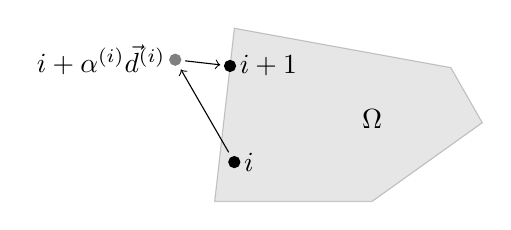
\begin{tikzpicture}
        \draw [thin, draw=black, fill=gray, opacity=0.2] (0,0) -- (.25,2.2) -- (3,1.7) -- (3.4,1) -- (2,0) -- cycle;
        \node [anchor=west] at (.25,.5) {$\mlei{i}$};
        \node (a) at (.25,.5){};
        \filldraw[black] (.25,.5) circle (2pt);
        \node [anchor=east] at (-.5,1.8) {$\mlei{i} + \alpha^{(i)} \vec{d}^{(i)}$};
        \node (b) at (-.5, 1.8){};
        \filldraw[gray] (-.5, 1.8) circle (2pt);
        \node (c) at (0.195563, 1.72096) {};
        \filldraw[black] (0.195563, 1.72096) circle (2pt);
        \node [anchor=west] at (0.195563, 1.72096) {$\mlei{i+1}$};
        \node at (2, 1.05) {$\mathlarger{\mathlarger{\Omega}}$};
        \draw[->] (b) to (c);
        \draw[->] (a) to (b);
    \end{tikzpicture}
\end{figure}

In \cref{alg:mle_search}, $\vec{d}^{(i)}$ is a unit vector denoting a \emph{promising} direction in which to search for a better solution than $\mlei{i}$. The Fisher scoring algorithm is a slight variation of Newton-Raphson\footnote{If the \emph{observed} information matrix is used instead of the \emph{expected} information matrix, the Fisher scoring algortihm is equivalent to Newton-Raphson.} in which
\begin{equation}
    \vec{d}^{(i)} = \infomatrx^{-1}\left(\mlei{i} \right) \score\left( \mlei{i} \right)\,.
\end{equation}
The scalar $\alpha^{(i)} > 0$ is the distance to move from point $\mlei{i}$ to generate the next point, $\mlei{i+1}$. Most naturally, the solution to
\begin{equation}
    \alpha^{(i)} = \argmax_{\alpha > 0} \ell(\mlei{i} + \alpha \cdot \vec{d}^{(i)})    
\end{equation}
is desired, e.g., using \emph{Golden Section} line search to find an approximate solution. Finally, the iterations are repeated until some \emph{stopping criteria} is satisfied. Most naturally, this is given by
\begin{equation}
    \| \score(\mlei{i}) \| < \epsilon\,,
\end{equation}
signifying a stationary point has been reached.

\chapter{Generic joint distribution}
\label{appendix:generalized_general_joint_likelihood_cand}
We assume the distribution of $\RV{W}$ does not carry information about the true parameter index $\tparam\sysparamvec$. By the axioms of probability, the joint distribution of $\rvcand$, $\sv$, and $\RV{W}$ is given by
\begin{equation}
\begin{split}
\pdf_{\rvcand, \sv, \RV{W}}(\cand, t, w \given \tparam\sysparamvec) &=\\ &\!\!\!\!\!\!\pmf_{\rvcand \given \sv, \RV{W}}(\cand \given t, w, \tparam\sysparamvec) \pmf_{\RV{W} \given \sv}(w \given t) \spdf(t \given \tparam\sysparamvec)\,.
\end{split}
\end{equation}

Since $\RV{W}$ carries no information about the true parameter index $\tparam\sysparamvec$, the maximum likelihood estimate $\mleu$ is independent of the distribution of $\RV{W}$.
\begin{proof}
\begin{equation}
\begin{split}
    \mleu &= \argmax_{\sysparamvec}
        \ell(\sysparamvec \given \mfso)\\
        &= \argmax_{\sysparamvec} \Biggl[ \sum_{i=1}^{n}
        \ln \pmf_{\rvcand \given \sv, \RV{W}}\left(\cand_i \given t_i, \Card{\cand_i}, \sysparamvec\right)\\
        &\qquad+ \sum_{i=1}^{n} \ln \spdf\left(t_i \given \sysparamvec\right) + \underbrace{\sum_{i=1}^{n} \ln \pmf_{\RV{W} \given \sv}\left(\Card{\cand_i} \given t_i \right)}_{\text{constant}}\Biggr]\,,
\end{split}
\end{equation}
where the last term is constant with respect to $\sysparamvec$ and may be dropped from the maximum likelihood equation without changing the point that maximizes the likelihood.
\end{proof}

The sampling distribution of $\mleu$ is a function of $\mfs$ (as opposed to a particular realization), and since $\mfs$ is a function of $\RV{W}$ (the distribution of the cardinality of candidate sets), the sampling distribution of $\mleu$ is also a function of $\RV{W}$.

Given a statistical model, the asymptotic sampling distribution of the maximum likelihood estimator is nearly automatic. The most taxing (and uncertain) part is the \emph{model selection}. Since we may not have much confidence in any particular model of the joint distribution of $\RV{W}$ and $\sv$, the \emph{expected} information matrix is sketchy. In general, the \emph{observed} information matrix is preferred. The sampling distribution of $\mleu$ converges in distribution to a multivariate normal with a mean given by $\tparam\sysparamvec$ and a variance-covariance given by the inverse of the \emph{observed} information matrix, written
\begin{equation}
    \sampdu \xrightarrow{d} \mvn\left(\tparam\sysparamvec, \observedn^{-1}\left(\tparam\sysparamvec \given \mfs\right)\right)\,.
\end{equation}

If an accurate distribution of $\RV{W} \given \sv = \ti$ could be constructed such that it is dependent on $\tparam\sysparamvec$, then the distribution of $\RV{W}$ in a sample carries extra information about $\tparam\sysparamvec$. A plausible model of $\RV{W}$ would depend upon the entropy of $\RV{K} \given \sv = \ti$.
\end{document}
